\subsection*{Exercise 3}
\boldmath\textbf{Is there a function $f: \nat \rightarrow \nat$ such that every $f(k)$-edge-connected graph is $k$-connected? Justify your answer.\\
\linebreak}
\unboldmath
If we have a graph $G$ that is $f(k)$-edge connected, there is no function that guarantees that the resulting graph is $k$-connected for any $G$. This is the case in graphs that have cut vertices (a cut vertex is a vertex whose removal increases the number of components of the graph). \\
\linebreak 
In the case of a graph with 1 or more cut vertices, the edge connectivity can be arbitrarily high, but the graph remains 1-connected. Take, for example a graph consisting of two complete graphs $K^1_n$ and $K^2_{n'}$ with a single vertex in common (this is then the cut vertex). See, for example, \ref{fig:wrong}, here $K^1_4 = \{v1, v5, v6, v7\}$ and $K^2_4 = \{v2, v3, v4, v5\}$. The two graphs share vertex $v5$. \\
\linebreak
This means that even for some graph with a very high edge-connectivity, and so a high $f(k)$ value, $k$ is still equal to 1. We cannot define a function such that the $k = 1$ and $f(k)$ is some value irrespective of the vertex connectivity. In conclusion, we cannot define a function $f: \nat \rightarrow \nat$ such that every $f(k)$-edge-connected graph is $k$-connected. \qed
\begin{center}
    \begin{figure}[h]
        \centering
        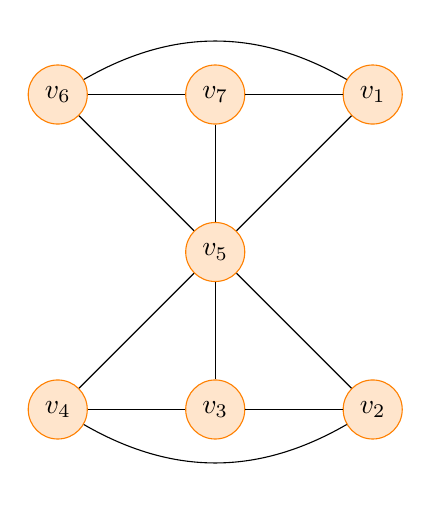
\begin{tikzpicture}
        \tikzset{
            dep/.style={circle,minimum size=0.75cm,fill=orange!20,draw=orange},
            vc/.style={circle, minimum
            size=0.75cm, fill=blue!20, draw=blue},
            c1/.style={-},
            c2/.style={dotted, purple, line width=2},
            c3/.style={dotted, black, line width=2},
            c4/.style={-, out=90, in=145}
            }

            \node[dep] (n1) at (1,2) {$v_1$};
            \node[dep] (n2) at (1,-2) {$v_2$};
            \node[dep] (n3) at (-1,-2) {$v_3$};
            \node[dep] (n4) at (-3,-2) {$v_4$};
            \node[dep] (n5) at (-1,0) {$v_5$};
            \node[dep] (n6) at (-3,2) {$v_6$};
            \node[dep] (n7) at (-1,2) {$v_7$};
            
            \draw[c1] (n1) to[above](n5);
            \draw[c1] (n5) to[above](n2);
            \draw[c1] (n2) to[above](n3);
            \draw[c1] (n3) to[above](n5);
            \draw[c1] (n3) to[above](n4);
            \draw[c1] (n4) to[above](n5);            
            \draw[c1] (n5) to[above](n6);            
            \draw[c1] (n6) to[above](n7);            
            \draw[c1] (n7) to[above](n5);            
            \draw[c1] (n7) to[above](n1);
            \draw[c1] (n6) to[bend left](n1);
            \draw[c1] (n2) to[bend left](n4);
        \end{tikzpicture}
        \caption{2-edge-connected 1-connected graph}
        \label{fig:wrong}
    \end{figure}
\end{center}